\documentclass[12pt]{exam}

\usepackage{amsmath, amssymb, amsthm, multicol}
\usepackage{graphicx}
\usepackage{textcomp}
\usepackage{tikz}

\newcommand{\vtx}[2]{node[fill,circle,inner sep=0pt, minimum size=4pt,label=#1:#2]{}}
\newcommand{\va}[1]{\vtx{above}{#1}}
\newcommand{\vb}[1]{\vtx{below}{#1}}
\newcommand{\vr}[1]{\vtx{right}{#1}}
\newcommand{\vl}[1]{\vtx{left}{#1}}
\renewcommand{\v}{\vtx{above}{}}

\def\d{\displaystyle}
\def\matrix#1{\begin{bmatrix}#1\end{bmatrix}}
\def\b{\mathbf}
\def\R{\mathbb{R}}
\def\Z{\mathbb{Z}}
\def\N{\mathbb{N}}
\def\and{\wedge}
\def\imp{\rightarrow}
\def\inv{^{-1}}
\def\st{~:~}



%\pointname{pts}
\pointsinmargin
\marginpointname{pts}
\marginbonuspointname{pts}
\addpoints
\pagestyle{head}
 % \printanswers

\firstpageheader{Math 228}{\bf Quiz 10}{Wednesday, November 15}


\begin{document}

%space for name
 \noindent {\large\bf Name:} \underline{\hspace{2.5in}}
 \vskip 1em

Consider the graph drawn below:
\begin{center}
  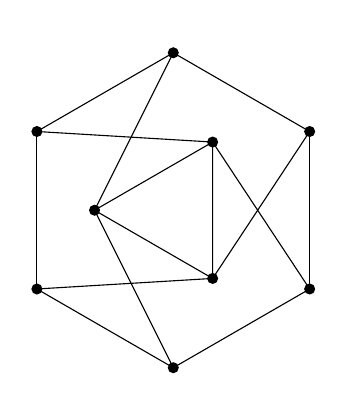
\begin{tikzpicture}
    \foreach \x in {0,...,5}{
    \coordinate (a\x) at (90-\x*60:2);
    \draw (a\x) \v -- (30-\x*60:2);
    }
    \coordinate (b1) at (60:1);
    \coordinate (b2) at (-60:1);
    \coordinate (b3) at (180:1);
    \draw (a0) -- (b3) \v -- (b2) \v -- (b1) \v -- (b3) -- (a3);
    \draw (a1) -- (b2) -- (a4) (a2) -- (b1) -- (a5);
  \end{tikzpicture}
\end{center}

\begin{questions}
\question[5] Note that the graph has 9 vertices and 15 edges.  Prove that the graph is NOT planar.
\begin{solution}
  Note, this problem turn out to be harder than intended.  If you just try to prove the graph is not planar using usual methods, you run into a problem:

  Assume that the graph is planar.  Then it would satisfy Euler's formula, so we have $9 - 15 + f = 2$, which gives $f = 8$ faces.  But we also know that $2e \ge 3f$ since each face is bordered by at least 3 edges, which are counted twice.  This means that $2\cdot 15 \ge 3\cdot 8$ or $30 \ge 24$.

  Alas, this is not a contradiction.  You can show that the graph is not planar, but to do so, you would want to see what happens when you delete the inner three edges.  This gives a graph that has 9 vertices and only 12 edges, so would have 5 faces.  However, now each face is bordered by at least 5 edges, so we get $2e \ge 5f$ which give $24 \ge 25$ which is a contradiction.  So the subgraph is not planar, which means the original graph is not planar either.
\end{solution}
\vfill
\question[5] Find the chromatic number of the graph.  Prove your answer is correctly by giving reasons you know the chromatic number cannot be larger or smaller than your answer.
\begin{solution}
  The chromatic number of the graph is 3.  We know it cannot be less than 3 because the graph contains a copy of $K_3$ (i.e., a triangle).  We know it cannot be larger than 3 because we can produce a 3-coloring:

  \begin{center}
    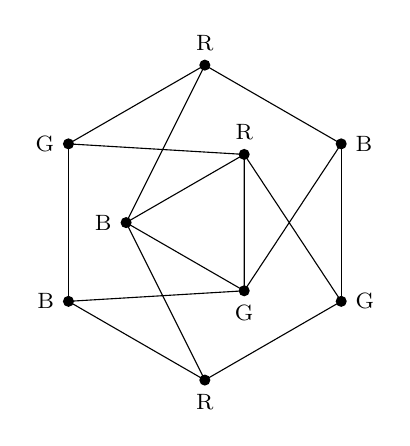
\begin{tikzpicture}
      \foreach \x in {0,...,5}{
      \coordinate (a\x) at (90-\x*60:2);
      \draw (a\x) -- (30-\x*60:2);
      }
      \coordinate (b1) at (60:1);
      \coordinate (b2) at (-60:1);
      \coordinate (b3) at (180:1);
      {\footnotesize
      \draw (a0) -- (b3) \vl{B} -- (b2) \vb{G} -- (b1) \va{R} -- (b3) -- (a3);
      \draw (a1) -- (b2) -- (a4) (a2) -- (b1) -- (a5);
      \draw (a0) \va{R} (a1) \vr{B} (a2) \vr{G} (a3) \vb{R} (a4) \vl{B} (a5) \vl{G};
      }
    \end{tikzpicture}
  \end{center}

\end{solution}
\vfill
\end{questions}
\end{document}
